\section{Introduction} \label{introduction}
Human action recognition is a challenging task for computer vision algorithms due to the large variabilities in video data caused by occlusions, camera motions, actor and scene appearances, among others. A popular current trend in action recognition methods relies on using local video descriptors to represent visual events in videos \cite{laptev2005, dollar2005, wang2011}. These features are usually aggregated into a compact representation, namely the bag-of-features (BoF) representation \cite{laptev2008}. The advantage of this simple representation is that it avoids difficult pre-processing steps such as motion segmentation and tracking. In the BoF representation, local descriptors are quantized using a pre-computed codebook of visual patterns. This representation combined with discriminative classifiers such as support vector machines (SVM), has been quite successful in recognizing human actions  in controlled scenarios \cite{blank2005, schuldt2004}. Due to its simplicity, BoF requires the use of strong, robust and informative features, which can be obtained reliably in such simplified scenarios. 

However, recent efforts have been made to collect more real-world video datasets (e.g. from movies and personal videos uploaded to video sharing websites  \cite{kuehne2011,  marszalek2009}), which are useful for evaluating human action recognition methods in more natural scenes. In fact, these datasets represent a challenge for existing BoF-based methods due to dynamic backgrounds, variations in illumination, and camera motions among other visual nuisances that can severely affect recognition performance.

\B{We need a section here on dense trajectories}


\begin{figure*}[ht]
\begin{center}
%\fbox{\rule{0pt}{1in} \rule{0.9\linewidth}{0pt}}
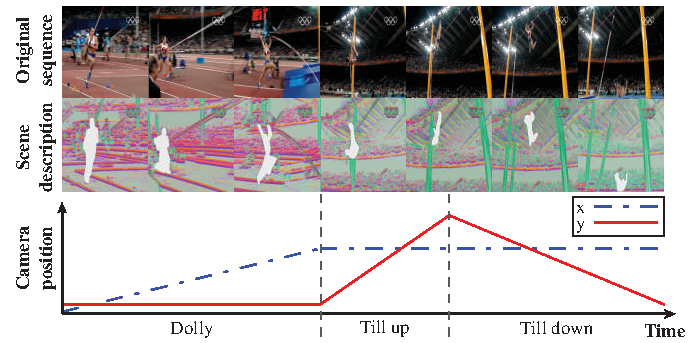
\includegraphics[width=0.98\linewidth]{fig/PullFigure.pdf}
\end{center}
\caption{Our pull figure. Endorse here.}
\label{fig:pull_figure}
\end{figure*}



\subsection{Related work}\label{subsec: related work}
A large amount of work has studied the problem of human action recognition in videos \cite{aggarwal2011}. In this section we overview some of the most relevant  previous work on the topic of feature extraction and action recognition in videos.

\paragraph{\textbf{Action Recognition}}The majority of action recognition methods relies on using local descriptors to represent visual events in videos \cite{laptev2005,dollar2005,wang2011}. Traditionally, these features are usually aggregated into a compact representation using a bag-of-features (BoF) representation framework \cite{laptev2008}. Moreover, recent studies show that using soft encoding techniques such as  Fisher Vectors \cite{perronnin2010} and VLAD \cite{jegou2012}, results in a boost for action recognition performance. These representations combined with discriminative classifiers such as support vector machines (SVM), has achieved tremendous success in action recognition. However, as discussed in \cite{xwang2013}, there are many details to be extensively explored, \ie feature extraction, feature pre-procesing, codebook generation, feature encoding and pooling and normalization. In this paper, we handle some of the current limitations on feature extraction.

\paragraph{\textbf{Feature Extraction.}} When applied to videos with substantial camera motion, traditional video features tend to generate a large number of features that are mostly related to the camera motion. In order to overcome this issue, Wu \etal \cite{wu2011} propose the use of Lagrangian particle trajectories for action description in videos acquired with moving cameras. Their method compensates for the global camera motion and only extracts features that exhibit motion independent to the camera movement, outperforming traditional feature extraction algorithms. Park \etal \cite{park2013} use a weak video stabilization based on a coarse optical flow to isolate limb motion while canceling pedestrian translation and camera motion. Wang \etal \cite{wang2011} present a method for action recognition using dense sampling of point trajectories. Their method handles large camera motions by limiting the maximum length of tracked trajectories. In spite of their simplicity, these dense trajectory features display significant performance improvements compared to detect salient sparse spatio-temporal features \cite{laptev2005}.

A couple of approaches try to improve upon these dense trajectories. Jain \etal \cite{jain2013} propose a method to estimate more reliable trajectory features for action recognition. Their method obtains improvements on feature robustness by first decomposing optical flow into dominant and residual motions. Dominant motion is estimated using an affine model and subtracted from the computed optical flow to obtain the residual motion. Similarly, Improved Trajectories \cite{wang2013} stabilize features fitting a homography using RANSAC filtering matches points coming out from human movements. Their framework improve the performance of several motion descriptors \ie Trajectory Shape, HOF and MBH. While these methods show a significant improvement when canceling background/residual motions, surrounding cues are discarded ignoring information like the scene appearance and distinct global motions correlated with specific actions.\\
A small number of works have studied the contribution of background and contextual information. Marszalek \etal \cite{marszalek2009} incorporate context information from movie scripts for human action recognition. Their method exhibit an important improvement when modeling the relations between actions and scenes based on textual co-occurrence. While such textual co-occurrence helps recognition, they are restricted only to certain source where scripts are available. In \cite{ikizler2010}, multiple feature channels are integrated from different source of information \ie human motion, scene information and objects. However, this approach uses a global description to describe scene properties \cite{oliva2001}. Rather than computing a holistic representation of the spatial envelope, we prefer to compute descriptor only from background regions. 

Our goal is to aggregate surrounding features that helps human actions representation. We are motivated due to the fact that most of videos are filmed with an intention. We encode this intention with a weak model for the camera movement computing a Fundamental Matrix over each pair of frames. Under the best of our knowledge any previous work focuses on correlating the film intention with actions.








%A large amount of work has studied the problem of human action recognition in videos \cite{Aggarwal2011}. In
%this section we overview some of the most relevant previous work on the topics of video stabilization, video
%feature extraction and action recognition in videos.
%
%A common methodology for video stabilization relies on estimating the global camera motion. One approach for
%this estimation computes sparse visual features \cite{Brown2003,Capel1998, Zoghlami1997} such as corners
%\cite{Censi1999} and estimates a warping matrix between consecutive frames. Others prefer to use all pixels
%in the image to compute an alignment \cite{Lucas1981, Matsushita2006}, but tend to suffer under-fitting due
%to local outliers. An alternative methodology defines a model for camera motion
%\cite{Buehler2001,Hansen1994} and uses multiple frames to estimate its parameters. Unfortunately, there is a
%large variation in camera motions and it is difficult to capture them in a single model. Once the camera
%motion is estimated, most algorithms use it to perform image alignment or warping \cite{szeliski2006image}.
%Unfortunately, warping usually introduces empty image regions in the aligned image. These areas may be
%recovered using impainting methods \cite{Wexler2004} at a high computational cost. Finally, instead of fully
%stabilizing sequences, \cite{Gleicher2008,GrundmannKwatra2011} propose to simulate professional camera
%motion in videos taken with handheld cameras. Unfortunately, not all camera motion is removed and the
%application of these methods to action recognition is limited. Most related to our approach, Park \etal
%\cite{Park2013} recently show how the use of weak video stabilization based on a coarse optical flow can
%lead to improved pedestrian detection in videos. Their goal is to isolate limb motion while cancelling
%pedestrian translation and camera motion. In this paper, we explore the extension of this technique and its
%applicability to feature extraction for action recognition.
%In another line of work, researchers have studied the issue of extracting video features for recognition
%that are robust to camera motion \cite{Jain2013,Gross2012,Wu2011a}. When applied to videos with large camera
%movement, traditional video feature extraction methods tend to generate a large number of features that are
%mostly related to the camera motion \cite{Dollar2005, Laptev2005, WangCVPR2011}. In order to overcome this
%issue, Wu \etal \cite{Wu2011a} propose the use of Lagrangian particle trajectories for action description in
%videos acquired with moving cameras. Their method compensates for the global camera motion and only extracts
%features that exhibit motion independent to the camera movement, outperforming traditional feature
%extraction algorithms. Matikainen \etal \cite{Matikainen2009} present a technique for action recognition
%with quantized trajectories of tracked features. More recently, Wang \etal presents a method for action
%recognition using dense sampling of point trajectories \cite{WangCVPR2011}. Their method handles large
%camera motions by limiting the maximum length of tracked trajectories. In spite of their simplicity, these
%dense trajectory features achieved state-of-the-art performance in bench-marking datasets. In order to
%improve upon these dense trajectories, Jain \etal \cite{Jain2013} propose a method to estimate more reliable
%motion features for action recognition. Their method obtains improvements on feature robustness  by first
%decomposing optical flow into dominant and residual motions. Dominant motion is estimated using an affine
%model and subtracted from the computed optical flow to obtain the residual motion. This information is then
%used to compute local motion descriptors. While the method is simple and improves recognition performance,
%residual and dominant motion estimations are not reliable when the dominant motion is related to the actor.
